\section{私有继承}
我们先来看看私有继承的相关知识。至于公开继承,我们的下一章几乎都是在借助它来进行讲解,所以现在就先不谈了。\par
与公开继承不同,私有继承一般不用来表示``属与种''的关系(Is-a relationship)。这是因为,在私有继承的条件下,基类的公有成员也只能作为派生类的私有成员存在,对外完全不可见。举个例子吧,所有的狗都会吠,所以我们应该把它作为狗的共性,置于 \lstinline@Dog@ 类下。
\begin{lstlisting}
class Dog {
    //...
public:
    void bark() {} //吠叫本领
};
class Husky : public Dog { /*...*/ };
class Retriever : public Dog { /*...*/ };
\end{lstlisting}
如果是公开继承的话,\lstinline@Husky@ 和 \lstinline@Dog@ 类的对象可以在外部调用基类的 \lstinline@bark@ 成员函数。这样体现的正是``派生类对象也是基类对象''的效果。\par
但假如是私有继承呢?比如说这么写吧:
\begin{lstlisting}
class Husky : Dog { /*...*/ }; //默认按私有方式继承
\end{lstlisting}
这就会出现一个问题:\lstinline@Dog::bark()@ 成为 \lstinline@Husky@ 的私有成员,它只对内可见,对外不可见。所以对外来说,相当于 \lstinline@Husky@ 类的对象没有吠叫本领,这显然是不合理的!
那么私有继承适合表示什么关系呢?我们来看一眼这个例子:
\begin{lstlisting}
class string { //class的默认成员访问权限是private,所以private可省略
    class Arr {
        char *_p;
    public:
        Arr(char* ptr = {nullptr}) : _p {ptr} {} //Arr的构造函数
        char*& p() { return _p; } //当arr不是常量时调用
        const char* p()const { return _p; } //当arr是常量时调用
    } _arr {new char[_cap]}; //象征指针的成员,默认用new char[_cap]初始化
    //...
\end{lstlisting}
读者应该对此比较熟悉,这是我们在第八章中讲讲解过的 \lstinline@string@ 类,这里是一个代码片段。请你想一想,这里的 \lstinline@Arr@ 类对象 \lstinline@_arr@ 是否满足以下特点:
\begin{itemize}
    \item \lstinline@_arr@ 的 \lstinline@public@ 成员对 \lstinline@string@ 来说好像是私有的\footnote{虽然这里声称``\lstinline@_arr@ 的成员也是 \lstinline@string@ 类的成员''显得不太合理,但我们讨论的只是可见性。},它们对 \lstinline@string@ 类来说可见,但对 \lstinline@string@ 以外的部分来说完全不可见。
    \item \lstinline@_arr@ 的 \lstinline@private@ 成员对 \lstinline@string@ 来说是不可见的。
\end{itemize}
而这个特点和私有继承是很相似的:
\begin{itemize}
    \item 基类的 \lstinline@public@ 成员对派生类来说是私有的。它们对派生类来说可见,但对外完全不可见。
    \item 基类的 \lstinline@private@ 成员对派生类来说是不可见的。\footnote{如果你认为基类的私有成员对派生类来说也属于成员,那么这些成员是``不可见成员'';如果你认为基类的私有成员对派生类来说不属于成员,那么一切顺理成章。}
\end{itemize}
私有继承表示的正是这种关系:一个对象是另一对象的一部分,\lstinline@_arr@ 是 \lstinline@string@ 对象的一部分。所以它表示的是``整体与部分''的关系(Has-a relationship)。\par
下面我就以 \lstinline@Arr@ 和 \lstinline@string@ 为例,改写上述代码:
\begin{lstlisting}
class Arr {
    char *_p;
protected:
    Arr(char *ptr = {nullptr}) : _p {ptr} {} //Arr的构造函数
    //单独的Arr对象可能没有意义,所以把构造函数设为protected,使其仅对派生类可见
public:
    char*& p() { return _p; } //当Arr的对象不是常量时调用
    const char* p()const { return _p; } //当Arr的对象是常量时调用
};
class string : private Arr { //private是默认的,可不写
    static constexpr std::size_t npos = -1;
    std::size_t _cap {0};
    std::size_t _size {0};
};
\end{lstlisting}\par
读者可以看到,在这种情况下,\lstinline@Arr@ 类的对象是内嵌在 \lstinline@string@ 对象中的。\lstinline@Arr@ 中公有和受保护成员的部分,包括构造函数和重载的 \lstinline@p@ 函数,在 \lstinline@string@ 类中都是私有的。至于 \lstinline@_p@,它在 \lstinline@string@ 类中完全不可见,只能通过 \lstinline@p()@ 来访问。\par
与原来那种定义方式(我们可以把它称为``组合方式'')不同,在私有继承方式下,这个内嵌的 \lstinline@Arr@ 对象没有名字;不过我们也不需要名字,直接把它当成自己的成员使用就行了。以下是对 \lstinline@string::swap@ 的改写,读者可以从中窥见它们在用法上的区别。
\begin{lstlisting}
//组合方式
void string::swap(string &str) {
    std::swap(_cap, str._cap);
    std::swap(_size, str._size);
    std::swap(_arr.p(), str._arr.p()); //p()不是自己的成员,需要借助_arr成员调用
}
//私有继承方式
void string::swap(string &str) {
    std::swap(_cap, str._cap);
    std::swap(_size, str._size);
    std::swap(p(), str.p()); //别见外,把p()当成自己的成员函数来调用
}
\end{lstlisting}\par
\subsection*{构造与初始化}
不过,因为这个内嵌的 \lstinline@Arr@ 对象没有名字,也没有显式的定义语句,所以我们不能像定义 \lstinline@_arr@ 时那样,为它提供一个默认成员初始值——不过,我们依然可以用初值列的方式来为它进行初始化:
\begin{lstlisting}
string::string(std::size_t count, char ch)
    : Arr {new char[count]}, _cap {count} //注意new char[count]
{
    for (; _size < count; _size++)
        at(_size) = ch;
}
\end{lstlisting}
这里我们初始化 \lstinline@Arr@ 对象的方式也是调用基类的构造函数,即 \lstinline@Arr{new char[count]}@ 这样。读者需要注意,在这里我们传入的参数不是 \lstinline@new char[_cap]@ 了,这是因为初值列的初始化顺序是\textbf{先基类成员,再派生类成员}。简单点说就是,基类成员 \lstinline@_p@ 会在派生类成员 \lstinline@_cap@ 之前初始化,所以这时就不能依赖 \lstinline@_cap@ 来为 \lstinline@_p@ 初始化,只能另谋出路。\par
如果我们依然想要用 \lstinline@_cap@ 来为 \lstinline@_p@ 初始化,那么我们不妨把它也改为基类的受保护成员。
\begin{lstlisting}
class Arr {
protected:
    std::size_t _cap;
    Arr(std::size_t cap,char *ptr = {nullptr}) 
        : _cap {cap}, _p {ptr} {} //Arr的构造函数
private:
    char* _p;
public:
    char*& p() { return _p; } //当Arr的对象不是常量时调用
    const char* p()const { return _p; } //当Arr的对象是常量时调用
};
\end{lstlisting}
但是这里存在另一个问题:C++17标准并没有保证不同访问权限的成员间的初始化顺序——换句话说,这样会把初始化变成一个未定义行为。为了预防这种情况的发生,我们还是要把 \lstinline@_arr@ 和 \lstinline@_p@ 都放在同一访问权限之下。\par
然而,如果把它们都放在 \lstinline@private@ 访问权限下,那么 \lstinline@_cap@ 就不能被派生类使用,这不符合我们的初衷;如果把它们都放在 \lstinline@protected@ 访问权限下,那么 \lstinline@_p@ 就可以被 \lstinline@string@ 类直接接触,起不到隔离的作用。为此,我们还需要更加取巧的方法才行,那就是——引用。
\begin{lstlisting}
class Arr {
    std::size_t ori_cap; //通过构造函数的初值列初始化
    char* _p = new char[ori_cap]; //默认成员初始值,依赖于ori_cap
protected:
    std::size_t &_cap = {ori_cap}; //_cap是对ori_cap的引用,置于protected下
    Arr(std::size_t cap = {0})
        : ori_cap {cap} {} //Arr的构造函数
public:
    char*& p() { return _p; } //当Arr的对象不是常量时调用
    const char* p()const { return _p; } //当Arr的对象是常量时调用
};
\end{lstlisting}
像这样,我们实际上初始化的是 \lstinline@ori_cap@,但是可以通过一个受保护的引用 \lstinline@_cap@ 来访问和修改这个值。这样,我们就在保证了正确初始化顺序的前提下,同时让 \lstinline@_p@ 和 \lstinline@_cap@ 都有了适当的访问权限。\par
接下来我们应该删去 \lstinline@string@ 类中的 \lstinline@_cap@ 定义,然后修改构造函数,把有关 \lstinline@_cap@ 的信息递交给 \lstinline@Arr@ 的构造函数来处理。
\begin{lstlisting}
string::string(std::size_t count, char ch) : Arr {count} {
    for (; _size < count; _size++)
        at(_size) = ch;
}
\end{lstlisting}
这里我们只需要显式调用 \lstinline@Arr@ 的构造函数就行了。至于 \lstinline@_size@ 的初始化,自有默认成员初始值来招待。\par
\subsection*{实操:适配\texttt{std::vector<int>}的\texttt{stack}类}
\lstinline@std::stack@ 是一种容器适配器\footnote{容器适配器(Container Adapter),是一种在特定容器类型上提供特定接口的数据结构,它们通过包装底层容器(如数组或链表)来提供特定的功能。},用来表示``栈''这个数据结构。\par
\textbf{栈(Stack)}是一种数据结构,它只支持两种基本的修改操作:从末端堆入数据(Push),或者从末端移出数据(Pop),如图9.4所示。C++在 \lstinline@stack@ 库中定义了 \lstinline@std::stack@ 类模版,读者可以在 \href{https://en.cppreference.com/w/cpp/container/stack}{std::stack - cppreference.com} 中查到它支持的功能等有关信息。
\begin{figure}[htbp]
    \centering
    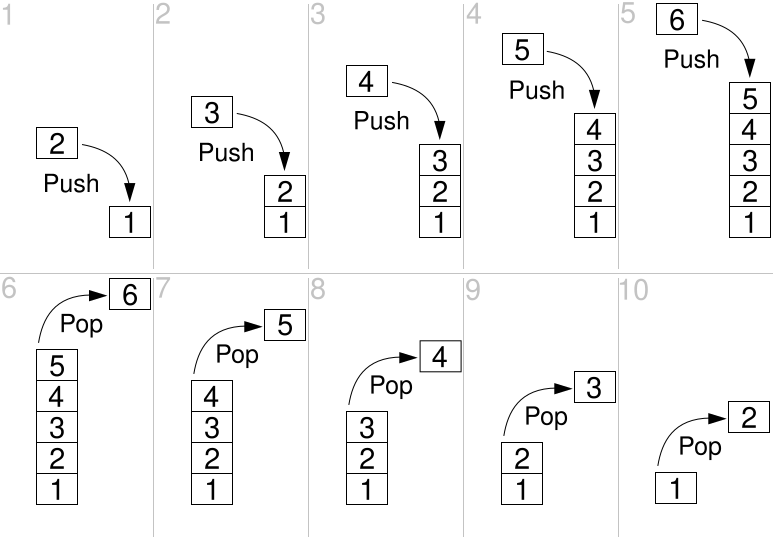
\includegraphics[width=.75\textwidth]{../images/generalized_parts/09_lifo_stack.png}
    \caption{栈的数据操作方式:从末端堆入、从末端移出}
    \footnotesize{图片来源:Wikipedia}
\end{figure}
关于 \lstinline@stack@ 类的具体实现,我们当然可以从一个裸的数组开始写起,但是这样太麻烦了。为此,我们可以让 \lstinline@stack@ 类内嵌一个 \lstinline@std::vector@ 对象,从而通过调用 \lstinline@std::vector@ 现成的成员函数来实现我们想要的基本功能。\par
注意,这些 \lstinline@std::vector@ 的功能仅限 \lstinline@stack@ 类内部使用;而对于外部来说,不是所有的 \lstinline@std::vector@ 成员函数都能调用。因此我们可以用私有继承的方式来实现,这样就保证了 \lstinline@std::vector@ 的公有成员都是 \lstinline@stack@ 的私有成员,从而起到屏障效果。
\begin{lstlisting}
class stack : private vector<int> { //private是默认的,可省略
    //...待补充
};
\end{lstlisting}
接下来我们就看一看,\lstinline@std::stack@ 有哪些功能,作为我们自己写 \lstinline@stack@ 类的参考。\par
\subsubsection*{功能简介}
\lstinline@std::stack@ 的内部功能是基于 \lstinline@std::deque@(双端队列)来实现的,但是我们还不熟悉这个容器,所以用 \lstinline@std::vector@ 来实现也未为不可。\par
\lstinline@std::stack@ 类的构造函数有很多,不过大多数都要用到我们还没学过的内容,所以一番挑拣下来,其实也就寥寥几个:
\begin{itemize}
    \item 默认构造函数将建立一个空的栈。
    \item 拷贝构造函数接收另一个同类\footnote{需要提醒,\lstinline@std::stack@ 是一个类模版而不是类。\lstinline@std::stack<int>@ 和 \lstinline@std::stack<double>@ 同属一个类模版,但却是两个不同的类。}对象。
    \item 有的构造函数接收一个 \lstinline@Container@ 类对象——对于我们来说,这个 \lstinline@Container@ 指的就是 \lstinline@std::vector<int>@。
    \item ……
\end{itemize}
\lstinline@std::stack@ 的析构函数也很简单。如果 \lstinline@stack@ 类没有什么动态内存操作的后顾之忧,那么我们不需要自行写一个析构函数,用默认的析构函数足够了。至于 \lstinline@std::vector<int>@ 中的动态内存空间,那应该是 \lstinline@std::vector<int>@ 的析构函数负责处理的。\par
赋值运算符很简单,只有从同类对象复制内容过来的版本。\par
\lstinline@top@ 成员函数可以返回当前栈的末尾变量的引用。而常成员函数的版本返回的是常量引用。\par
\lstinline@empty@ 返回一个 \lstinline@bool@ 变量,用来表示当前栈是否为空。\par
\lstinline@size@ 返回一个 \lstinline@std::size_t@ 变量,用来表示当前栈的数据量。\par
\lstinline@push@ 用来在栈的末端堆入数据;而 \lstinline@pop@ 正相反,用来在栈的末端移出数据。\par
\lstinline@swap@ 函数是我们的老朋友了。\par
比较运算符也还是老样子,做字典序比较就行了。\par
读者能感觉到这个项目比前面的 \lstinline@string@ 要简单多了,那么事不宜迟,我们马上来规划一下要怎么做吧。\par
\subsubsection*{规划}
我们还是按照先声明后定义的顺序来构建这段代码。除非定义部分很简单,否则我们都把它写在类外。\par
对于私有成员部分,我们有一个私有继承的 \lstinline@std::vector<int>@ 类内嵌对象,已经足够。\par
而在公有成员部分,我们首先需要定义构造函数:
\begin{lstlisting}
public:
    explicit stack() {} //什么也不做
    stack(const stack&); //拷贝构造函数
    explicit stack(const std::vector<int>&); //接收一个std::vector<int>对象
\end{lstlisting}
其中的两个函数被冠以 \lstinline@explicit@,这就限制了它们的隐式类型转换操作。其中的默认构造函数即便什么也不做,也会调用基类 \lstinline@std::vector<int>@ 的默认构造函数。\par
至于析构函数,我们没有必要自定义,直接用默认版本就足够了。\par
接下来是赋值运算符。
\begin{lstlisting}
public:
    stack& operator=(const stack&); //赋值运算符
\end{lstlisting}\par
然后是 \lstinline@top@ 函数。注意,它分为常成员函数版本和非常成员函数版本,其返回类型是不同的。
\begin{lstlisting}
    int& top() { return back(); } //调用std::vector<int>的back函数
    const int& top()const { return back(); } //常成员函数版本
\end{lstlisting}
在这个函数的定义中我们看到,我们是直接调用 \lstinline@back@ 函数来修改基类成员的。\lstinline@stack@ 函数内部并未定义 \lstinline@back@ 函数,所以根据名称查找规则\footnote{读者可以回忆一下我们在第七章第三节中讲过的关于``名称查找''的内容。对于继承关系来说,也有名称查找规则:如果在这个类中找不到这个名称,那么就去它的基类中查找。},它会找到 \lstinline@std::vector<int>@ 的 \lstinline@back@ 成员函数。\par
如果你想要避免的歧义,也可以通过作用域解析操作符来显式地指定我们要调用哪个成员函数:
\begin{lstlisting}
    int& top() {return std::vector<int>::back(); }
    //显式指定调用std::vector<int>的back成员函数
\end{lstlisting}\par
\lstinline@empty@ 成员函数和 \lstinline@size@ 成员函数也不难。唯独需要注意一点——
\begin{lstlisting}
    bool empty()const { return size(); } //调用谁的size函数?
    std::size_t size()const { return std::vector<int>::size(); }
    //调用std::vector<int>的size()函数
\end{lstlisting}
先来看看这个 \lstinline@size@ 成员函数。我们发现,这个函数的名字与 \lstinline@std::vector<int>::size()@ 相互冲突。如果我们直接写 \lstinline@size()@ 的话,编译器会根据名称查找规则,找到 \lstinline@stack::size()@,所以在这里就会发生 \lstinline@stack::size()@ 的无穷递归调用,进而发生错误。\par
为了解决这个问题,我们必须显式地让编译器知道我们真正想调用的是哪个函数,所以我们要写成 \lstinline@std::vector<int>::size()@。至于 \lstinline@empty@ 函数,我们可以有很多种实现方法。除了上文中调用 \lstinline@stack::size()@ 加隐式类型转换的方法以外,还有这些选择:
\begin{lstlisting}
    bool empty()const { return std::vector<int>::size(); }
    //调用std::vector<int>的成员函数,再隐式类型转换
    bool empty()const { return std::vector<int>::empty(); }
    //std::vector<int>也有empty()成员函数,可以直接用它
\end{lstlisting}
读者选其中一种来实现就可以了。\par
\lstinline@push@ 接收一个 \lstinline@const int&@ 参数,而 \lstinline@pop@ 不接收参数,所以这样写就行了。
\begin{lstlisting}
    void push(const int&); //堆入数据
    void pop(); //移出数据
\end{lstlisting}\par
\lstinline@swap@ 成员函数亦如此。
\begin{lstlisting}
    void swap(stack&); //交换内容
\end{lstlisting}\par
比较运算符还是一如既往地利用代码重用来实现。这里除了 \lstinline@std::lexicographical_compare@ 以外,我们还多了别的选择,我们稍后再讲。
\begin{lstlisting}
    bool operator<(const stack&)const;
    bool operator>(const stack&)const;
    bool operator<=(const stack&)const;
    bool operator>=(const stack&)const;
    bool operator==(const stack&)const;
    bool operator!=(const stack&)const; //六个比较运算符
\end{lstlisting}\par
\subsubsection*{实现}
接下来把没定义的成员函数定义一下。首先是构造函数和拷贝构造函数。
\begin{lstlisting}
stack::stack(const std::vector<int> &v) : std::vector<int>{v} {}
//构造函数
stack::stack(const stack &s) : std::vector<int>{s} {}
//拷贝构造函数
\end{lstlisting}
这里的构造函数调用了 \lstinline@std::vector<int>@ 的拷贝构造函数,用以为 \lstinline@stack@ 类内嵌的 \lstinline@std::vector<int>@ 对象初始化。而下面的拷贝构造函数就显得有些反常,它传入的参数是 \lstinline@stack@ 类的?\par
其实这是因为,基类与派生类之间可以进行隐式类型转换。我们会在下一章中讲解这方面的详细知识;现阶段读者只需要明白,\textbf{派生类的对象可以无风险地隐式类型转换成基类对象——得到的正是那个内嵌于派生类中的基类对象}\footnote{在类的内部,这个关系是成立的;对于公有继承来说,这个关系也成立。但是对于私有继承的派生类来说,在类外不允许这种隐式类型转换。}。所以这里传入的 \lstinline@s@ 会先隐式类型转换成 \lstinline@std::vector<int>@ 类型,然后用以构造。\par
\begin{lstlisting}
stack& stack::operator=(const stack &s) {
    if (this == &s) //防止自我赋值
        return *this;
    std::vector<int>::operator=(s);
    //调用std::vector<int>的赋值运算符,并借助隐式类型转换参数传递
    return *this;
}
\end{lstlisting}
在赋值运算符中我们也使用了相同的技巧。我们先是通过作用域解析运算符指定了要调用谁的赋值运算符,然后又通过 \lstinline@stack@ 到 \lstinline@std::vector<int>@ 的隐式类型转换成功地把参数传递过去了。\par
接下来提供 \lstinline@push@ 和 \lstinline@pop@ 函数的定义。\lstinline@std::vector@ 中并没有 \lstinline@push@ 和 \lstinline@pop@ 成员,所以我们定义函数时不需要担心出现重名问题,可以不必再使用作用域解析运算符。
\begin{lstlisting}
void stack::push(const int &val) {
    push_back(val); //将调用std::vector<int>::push_back
}
void stack::pop() {
    pop_back(); //将调用std::vector<int>::pop_back
}
\end{lstlisting}
当然,如果你愿意,也可以写成 \lstinline@std::vector<int>::push_back@ 这样。\par
\begin{lstlisting}
void stack::swap(stack &s) {
    std::vector<int>::swap(s);
}
\end{lstlisting}
\lstinline@swap@ 成员函数的定义也是这样进行的,这里就不再赘述。\par
\begin{lstlisting}
bool stack::operator<(const stack &s)const {
    return *this < static_cast<std::vector<int>>(s);
}
\end{lstlisting}
小于号这样定义就可以。需要注意,对于 \lstinline@std::vector@ 来说,小于号并不是成员函数,而是非成员函数,因此我们不能用成员函数的调用方法。\par
另外读者可能会对 \lstinline@*this<static_cast<std::vector<int>>(s)@\footnote{请读者留意,一些上古编译器会把两个半尖括号 \lstinline@>>@ 识别成右移位运算符。如果发生了这样的事情,读者只需在两个半尖括号之间加一空格,改写成 \lstinline@> >@ 就可以了。相似的情形还有两个半方括号 \lstinline@[[@ 这样的写法,可能会被编译器当作属性说明符,这时我们只需要加一空格就可以了。}这样的写法感到好奇——难道这样不会像我们在第二章第四节末尾所讲那样\footnote{我们曾就 \lstinline@static_cast<int>(a)*b@ 这个语法做过讨论,发现在这个类型转换的过程中,\lstinline@a@ 被转换为 \lstinline@int@ 型之后马上又被转换为 \lstinline@double@,结果并没有实现我们的目的。},\lstinline@s@ 被转换成 \lstinline@std::vector<int>@ 类型后又被转换成 \lstinline@stack@ 类型吗?其实不会,这是因为继承关系所带来的隐式类型转换是不平等的。派生类的对象可以无风险转换为基类对象\footnote{再次提醒,对于类内部来说才有这样的隐式类型转换关系;对于类外部来说就未必了。},但基类对象就不能隐式转换为派生类对象。所以对于 \lstinline@*this<static_cast<std::vector<int>>(s)@ 来说,只有一种可能的转换方式,就是二者都转换为 \lstinline@std::vector<int>@ 对象。\par
接下来的几个比较运算符就是小儿科了。
\begin{lstlisting}
bool stack::operator<(const stack &s)const {
    return *this < static_cast<std::vector<int>>(s);
}
bool stack::operator>(const stack &s)const {
    return s < *this;
}
bool stack::operator<=(const stack &s)const {
    return !(s < *this);
}
bool stack::operator>=(const stack& s)const {
    return !(*this < s);
}
bool stack::operator==(const stack &s)const {
    return !operator!=(s); //利用已经声明的stack::operator!=
}
bool stack::operator!=(const stack &s)const {
    return *this < s || s < *this; //比较运算符的优先级高于逻辑或运算符
}
\end{lstlisting}
好了,这样我们就完成了一个基本的 \lstinline@stack@ 类。\par
\subsection*{组合方式,还是继承方式?}
如果我们要表示一个类的私有对象,那么有两种方式可供我们进行选择:一种是在我们之前用的组合方式(Containment),一种是我们刚才看到的私有继承方式(Private inheritance)。\par
绝大多数程序员都会毫不犹豫地选择组合方式,因为:
\begin{itemize}
    \item 组合方式下,每个成员对象都有名字。我们可以很方便地知道哪个对象是什么、意味着什么,以及是哪个对象在调用成员函数——试想,我们刚才调用 \lstinline@size()@ 的时候很容易陷入到无穷递归的陷阱中;如果每个成员对象有各自的名字,那么我们一眼就可以看出我们正在调用的函数是什么,属于谁。
    \item 组合方式下,我们可以定义多个成员对象。虽然有些时候我们只需一个对象就够了——\lstinline@stack@ 正是这样的情形;但是如果我们需要内嵌多个对象,那么私有继承方式就不管用了,我们必须组合。
\end{itemize}
无论怎么说,这些优点都太显著,所以我们常常会忽略私有继承这种方式。\par
但是,私有继承方式也有它的些许优点:
\begin{itemize}
    \item 如果我们希望像 \lstinline@Arr@ 那样只把 \lstinline@p()@ 当作一个随机而变的成员对象来使用的话,定义一个 \lstinline@_arr@ 作为中介还是麻烦了点。不如通过继承方式,让 \lstinline@p()@ 成为真正意义上的成员。
    \item 在继承方式下,基类的受保护成员对派生类也可见,这就为我们在某些特定条件下写代码提供了便利。
    \item 继承方式还为多态提供了可能,我们会在下一节中讲到。
\end{itemize}\par
如果要我描述的话,我认为私有继承相较于组合方式来说,有点像 \lstinline@mutable@ 成员相较于普通成员——如果没有什么这方面的专门需求,就不要用它。总之我是不会在写 \lstinline@Dog@ 类的时候让它继承一个 \lstinline@unsigned@ 类和一个 \lstinline@double@ 类\footnote{一个类可以继承多个基类,这叫作多重继承。我们会在第十章讲解相关内容。},这种没有名字只有类型的事物,光是看上去就很让人困惑了。\par
